\chapter{Results}

We discuss the results obtained using the tool through a number of real world cases.
The first of these additionally serves as a comprehensive, didactic, example of how to use the tool. 

\section{Diagnosing a failing inspection test in \mono{Text}}

Hearkening back to \mono{inspection-testing} discussed in \cref{section:introduction_inspection_testing}, we put
ourselves in the shoes of a programmer who gets surprised by a failing inspection test and reason how we might
employ HsComprehension to diagnose the problem. 

To summarize, we expected that the function \mono{countChars} which counts the number of characters in a \mono{ByteString}
using a number of functions in the \mono{Text} library, will in its final form not actually construct a \mono{Text} value.

\paragraph{1. Isolate the problem}
Modules typically contain more than 1 function and during the core2core transformations many more auxiliary functions are
added, and many functions are inlined to produce exponentially more code. Despite the tool being designed with features to 
comprehend medium-sized modules, it is still most helpful to temporarily isolate the
failing test case into a separate module:

\begin{minted}{haskell}
{-# LANGUAGE TemplateHaskell #-}

module InspectionTests where

import Test.Inspection
import qualified Data.Text as T
import qualified Data.Text.Encoding as TE
import Data.ByteString

countChars :: ByteString -> Int
countChars = T.length . T.toUpper . TE.decodeUtf8

-- the failing test case
inspect $ 'countChars `hasNoType` ''T.Text
\end{minted}

The following error is produced by the build:

\begin{minted}{sh}
app/InspectionTests.hs:21:1: countChars `hasNoType` Data.Text.Internal.Text failed:
# ...
# 700 lines of core as seen at the end of the core2core pipeline
# ...
\end{minted}

700 lines of textual data is generated from just this one function!
It is also incomplete in the sense that it does not show the process that produced this final
artifact.

\paragraph{2. Creating a capture}

Because we only want to create a capture of this module, we can use an exported TemplateHaskell primitive
that registers the plugin for the current module only by simply adding the \mono{dumpThisModule} snippet 
anywhere at the toplevel: 

\begin{listing}[H]
\begin{minted}{haskell}
{-# LANGUAGE TemplateHaskell #-}
import HsComprehension.Plugin (dumpThisModule)

...

dumpThisModule
\end{minted}
\end{listing}

Following a successful build, we can bundle the generated artifacts to a zip archive by running:

\begin{listing}[H]
\begin{minted}{sh}
$ cabal run hs-comprehension-zip
Attempting to archive dump files in ./dist-newstyle/coredump-Default
Archiving 23 files
Created /home/hugo/repos/hs-comprehension/test-project/dist-newstyle/Default.zip
\end{minted}
\end{listing}

\paragraph{3. Finding the root cause}
We navigate to \href{https://core.hugopeters.me}{core.hugopeters.me} and upload the zip archive we just
produced.

\begin{figure}[H]
\centering
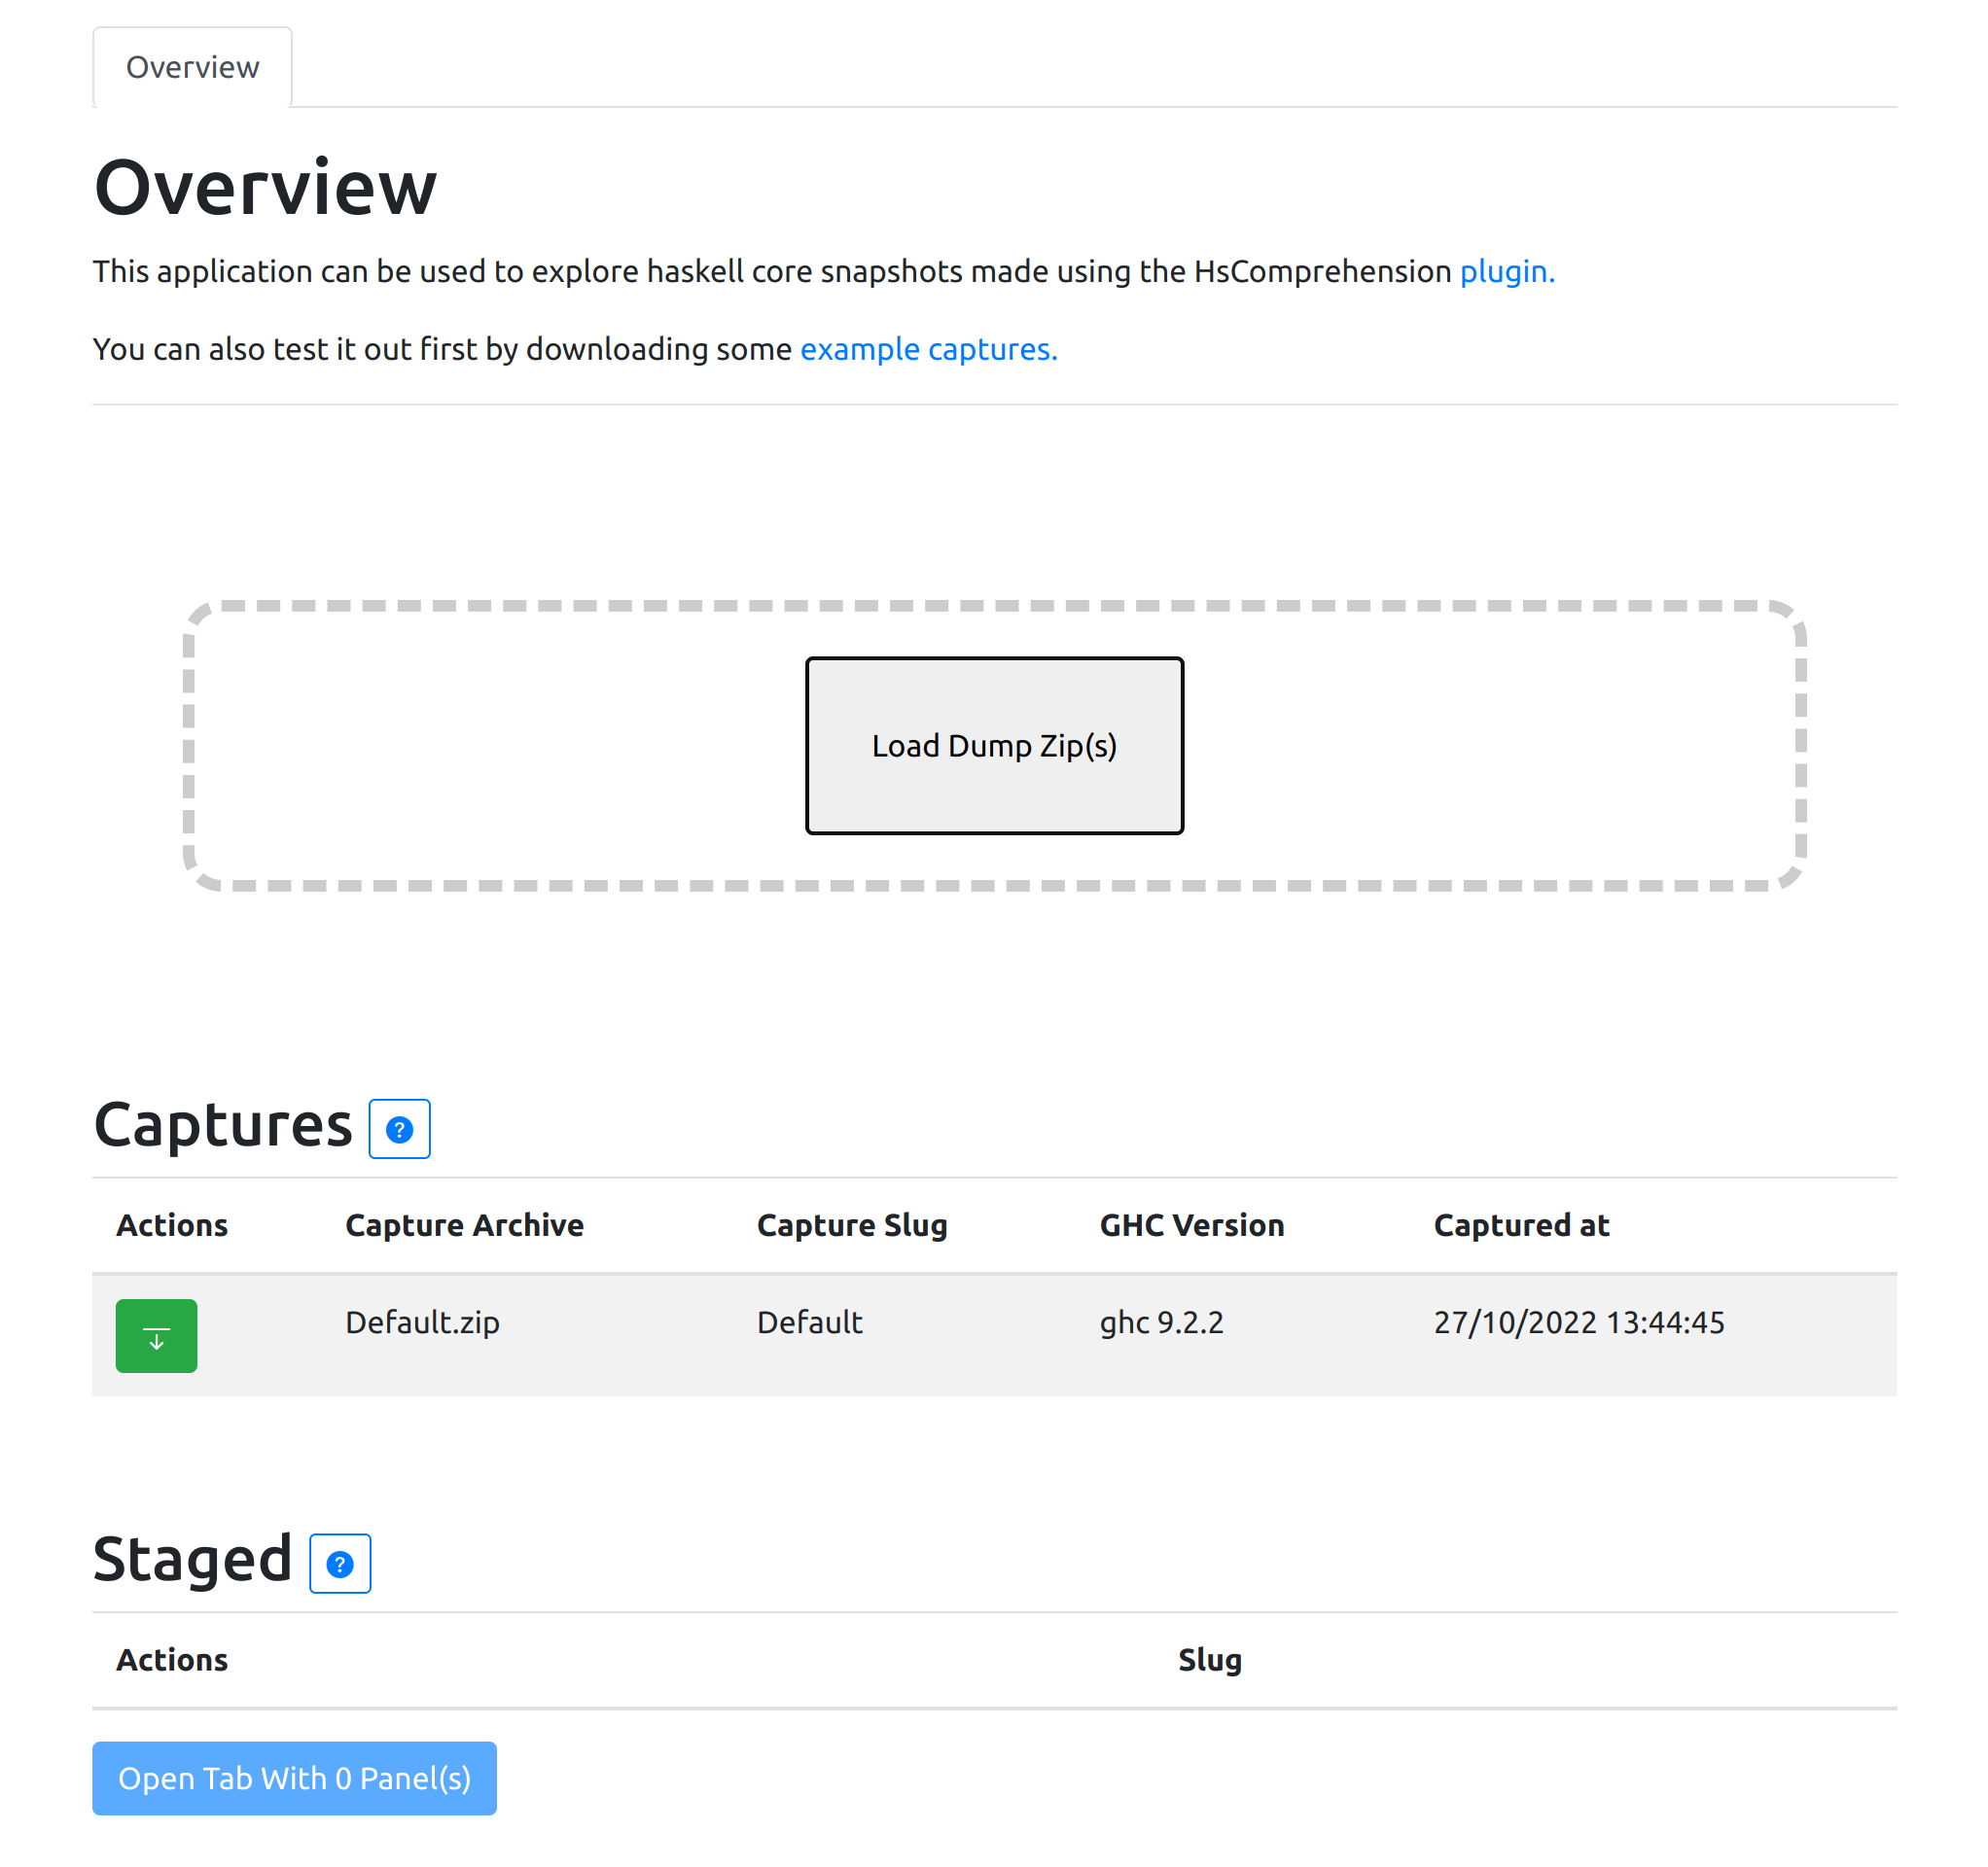
\includegraphics[width=0.8\textwidth]{figs/countchars_1.png}
\label{fig:countchars_1}
\end{figure}

We then click the green arrow to reference the capture in the staging area. Here we could elect to stage more
than one capture if we want to compare them. In this case we are only interested in the current situation, and so we
just open a single panel tab with this single capture


\begin{figure}[H]
\centering
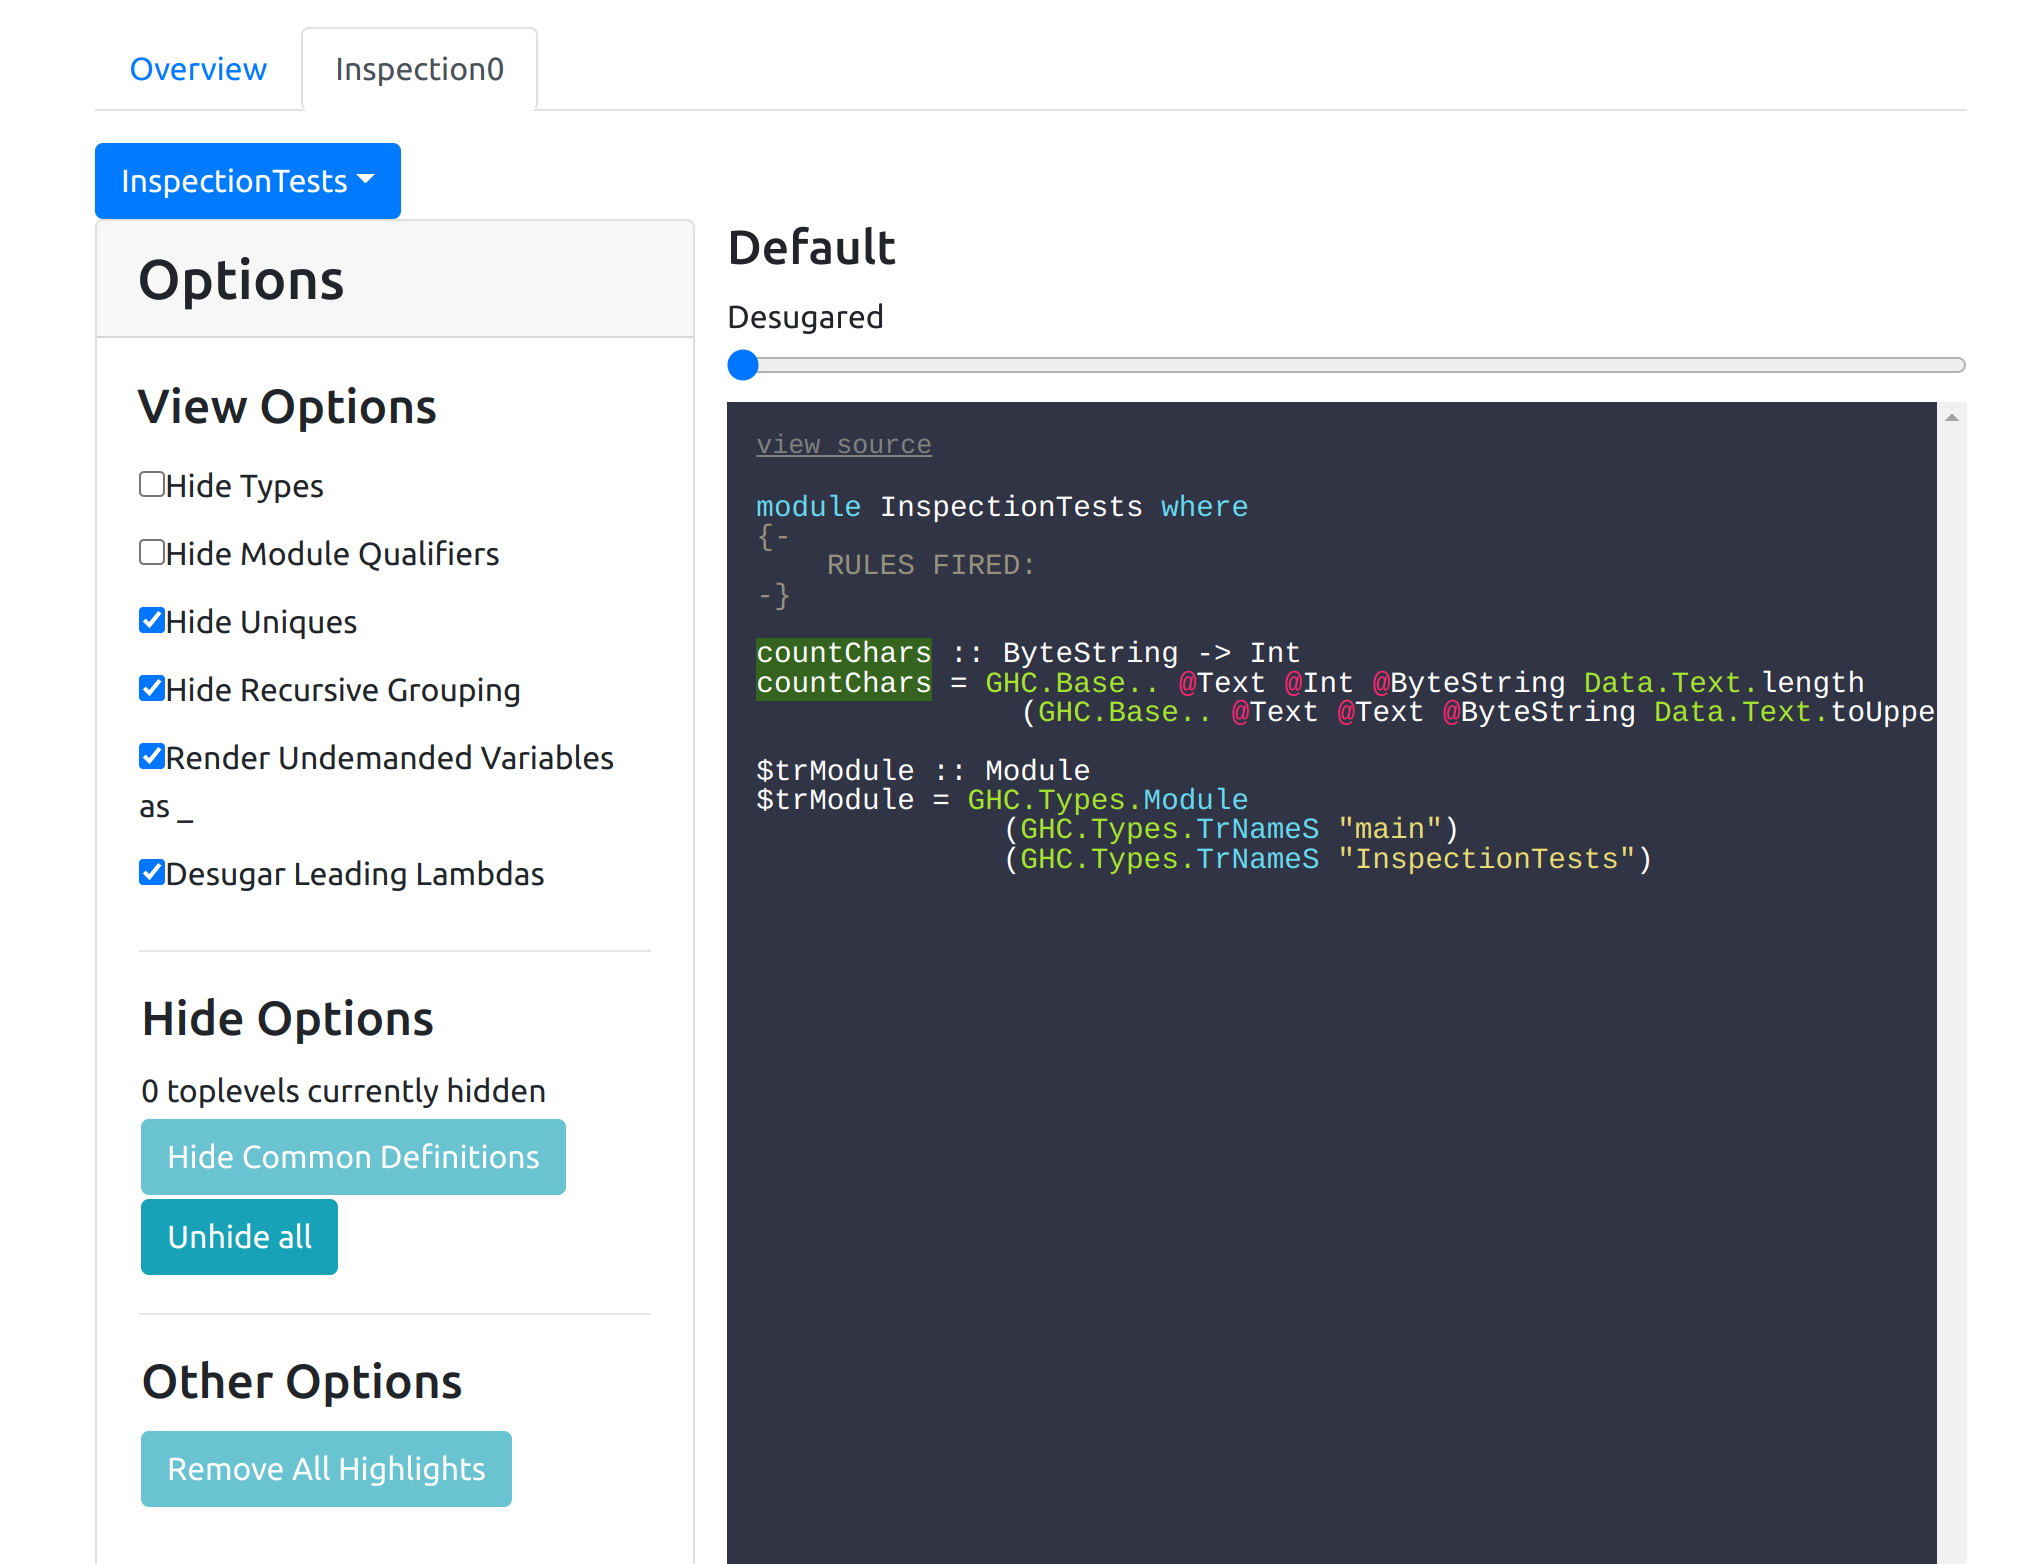
\includegraphics[width=0.8\textwidth]{figs/countchars_2.png}
\label{fig:countchars_2}
\end{figure}

On the left, are immediately presented with a number of viewing options. To the right we can see the rendered
Core, under influence of the view options. Above it a slider indicating that we are looking at the
Core in the desugared stage (so without any transformations yet applied). Scrolling this slider will reveal
the intermediate Core ASTs that were produced by the compiler. Whenever rewrite rules are fired they are included
as comments at the top of the module.

As you can see, the desugaring process has produced another top-level definition, namely \$\mono{trModule}. Since we
not care for anything but our \mono{countChars} function at this time, we can elect to filter out all other definitions,
including those that will be generated in the future: 

\begin{figure}[H]
\centering
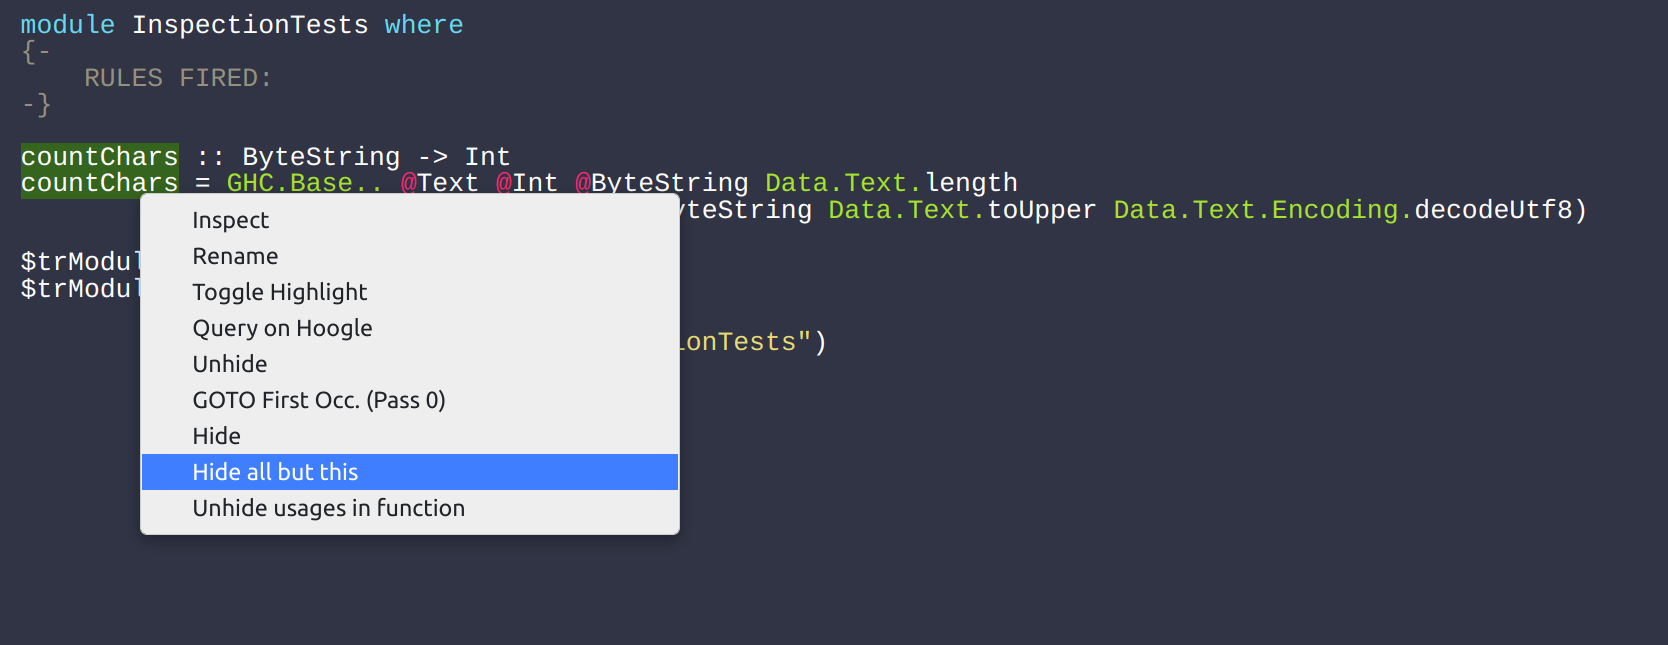
\includegraphics[width=0.8\textwidth]{figs/countchars_hideallbut.png}
\label{fig:countchars_3}
\end{figure}

If we then scroll all the way to the end, we get the same final Core AST as we saw in the error message. Granted,
we now have syntax highlighting and a slightly more readable representation, but it is still unwieldy. Using a basic string search we can find the needle in the haystack:

\begin{figure}[H]
\centering
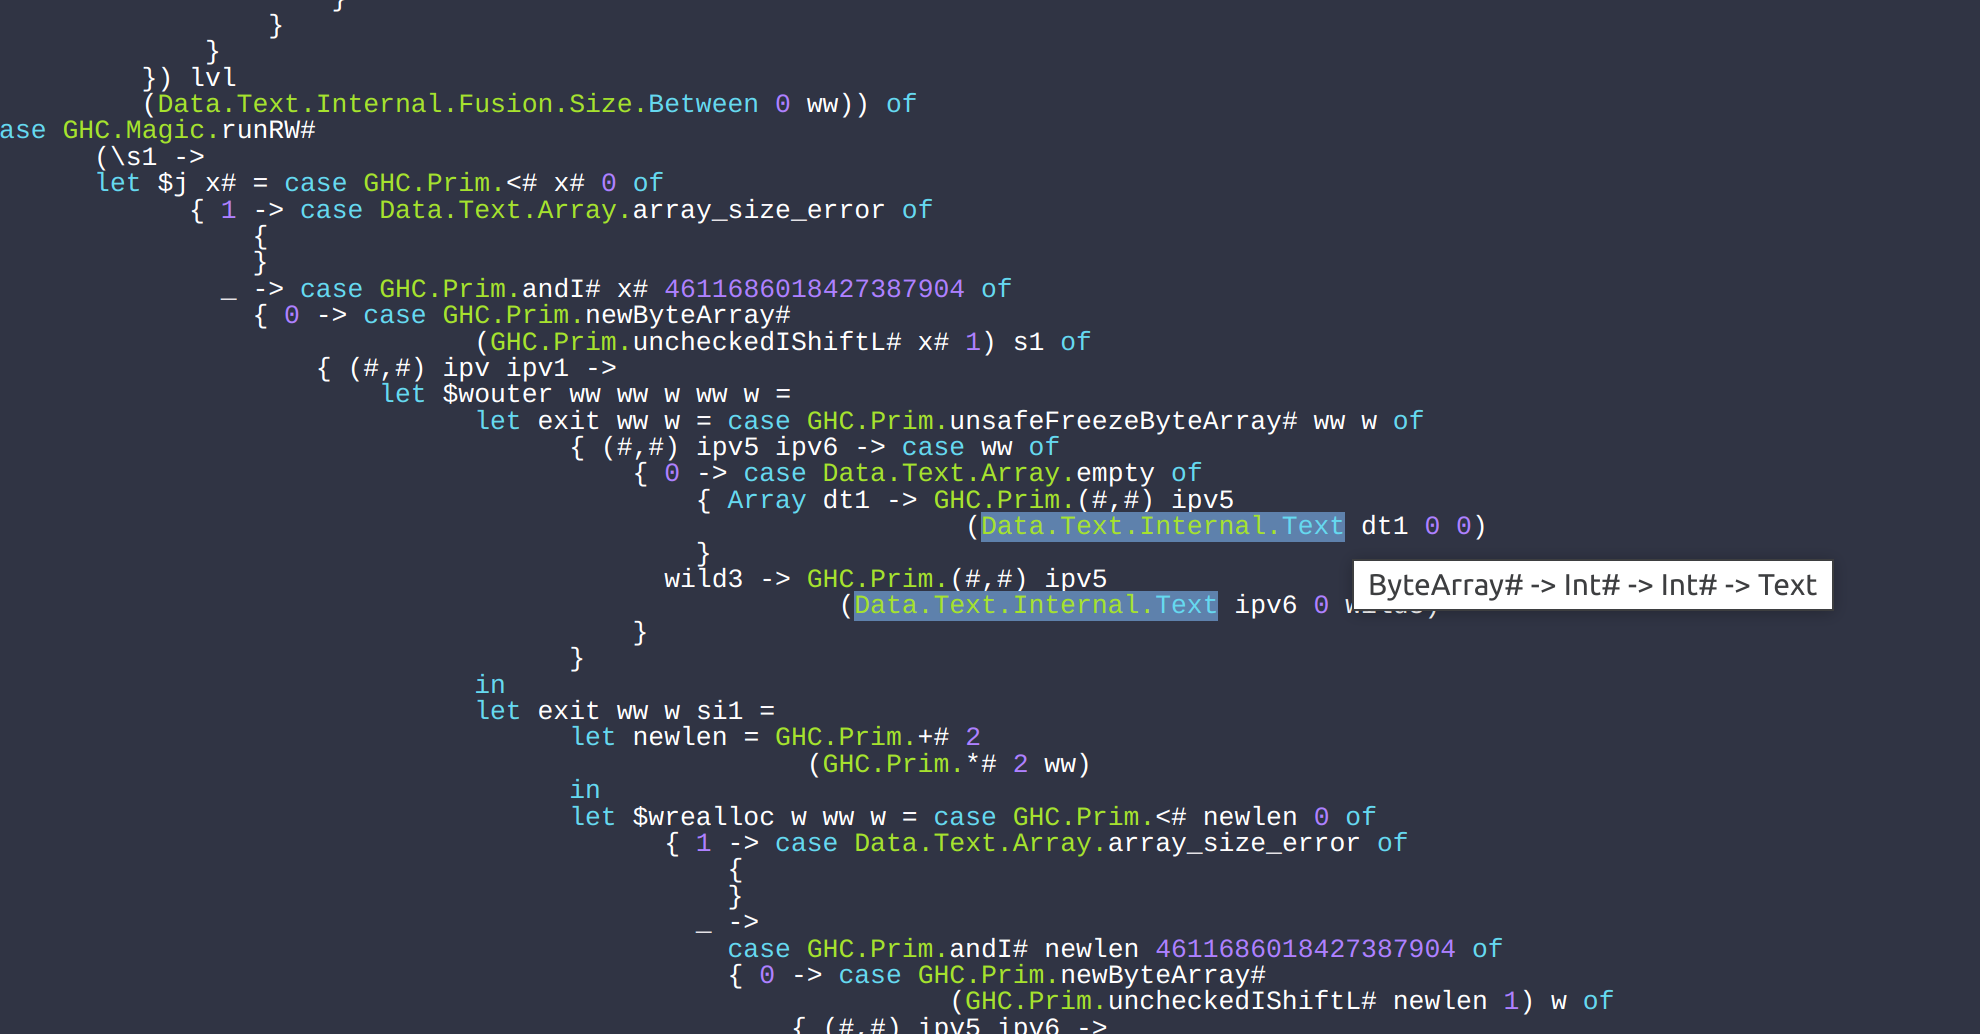
\includegraphics[width=0.8\textwidth]{figs/countchars_3.png}
\end{figure}

But we don't really care about finding the needle, but more so how it got it there.
Using the scroll bar we can go back in time to a moment before everything was inlined.
Specifically, we can go back to the first moment where no \mono{Text} constructor existed yet:

\begin{figure}[H]
\centering
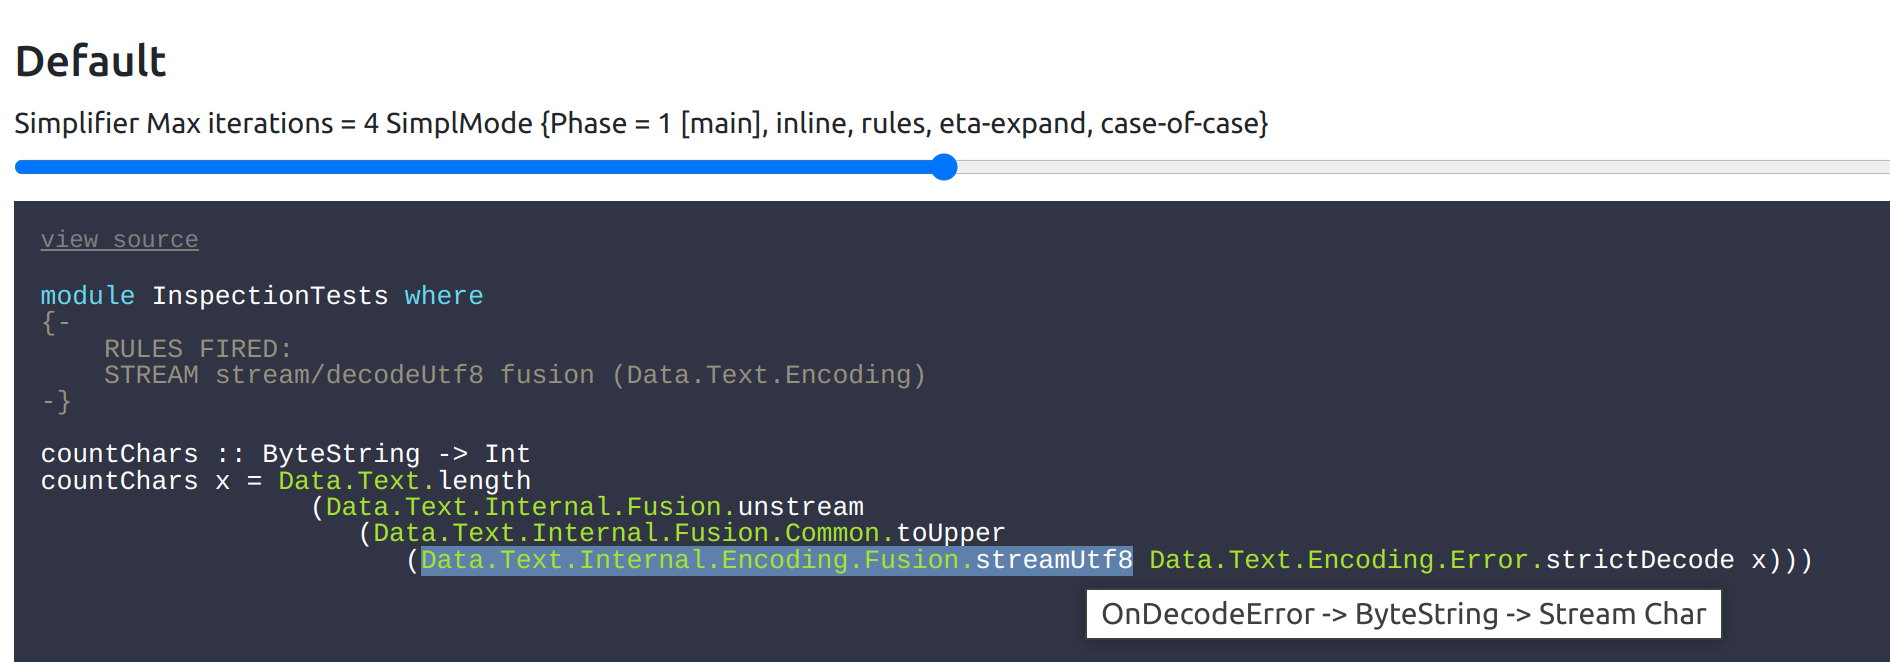
\includegraphics[width=0.8\textwidth]{figs/countchars_4.png}
\end{figure}

We find a far more manageable definition of \mono{countChars} that has partially been transformed to operate on streams (\mono{Stream Char}).
This is a concept to faciliate fusion based on the work of D. Couts et al. \cite{stream_fusion}, we will discuss its theory more
in depth in next section. For now, it is only important to realise that instead of embedding the
incoming \mono{ByteString} in a \mono{Text} value, we are converting to a \mono{Stream Char} first before \mono{unstream}
converts to an actual \mono{Text}. The argument that this is not necessary still holds because there conceivably exists a length
function for values of type \mono{Stream Char} as well. 

So we can conclude that the \mono{text}'s fusion machinery did not produce the optimal result because it is conceivable to find the
length of a stream directly using some alternative \mono{length :: Stream Char -> Int} function.

\paragraph{4. Back to the future}

Luckily, we were reliving someone else's experience, and we have the luxury of seeing how the situation unfolded.
So, what we can do is make another capture with a more recent version of the library, and compare the two:

\begin{figure}[H]
\centering
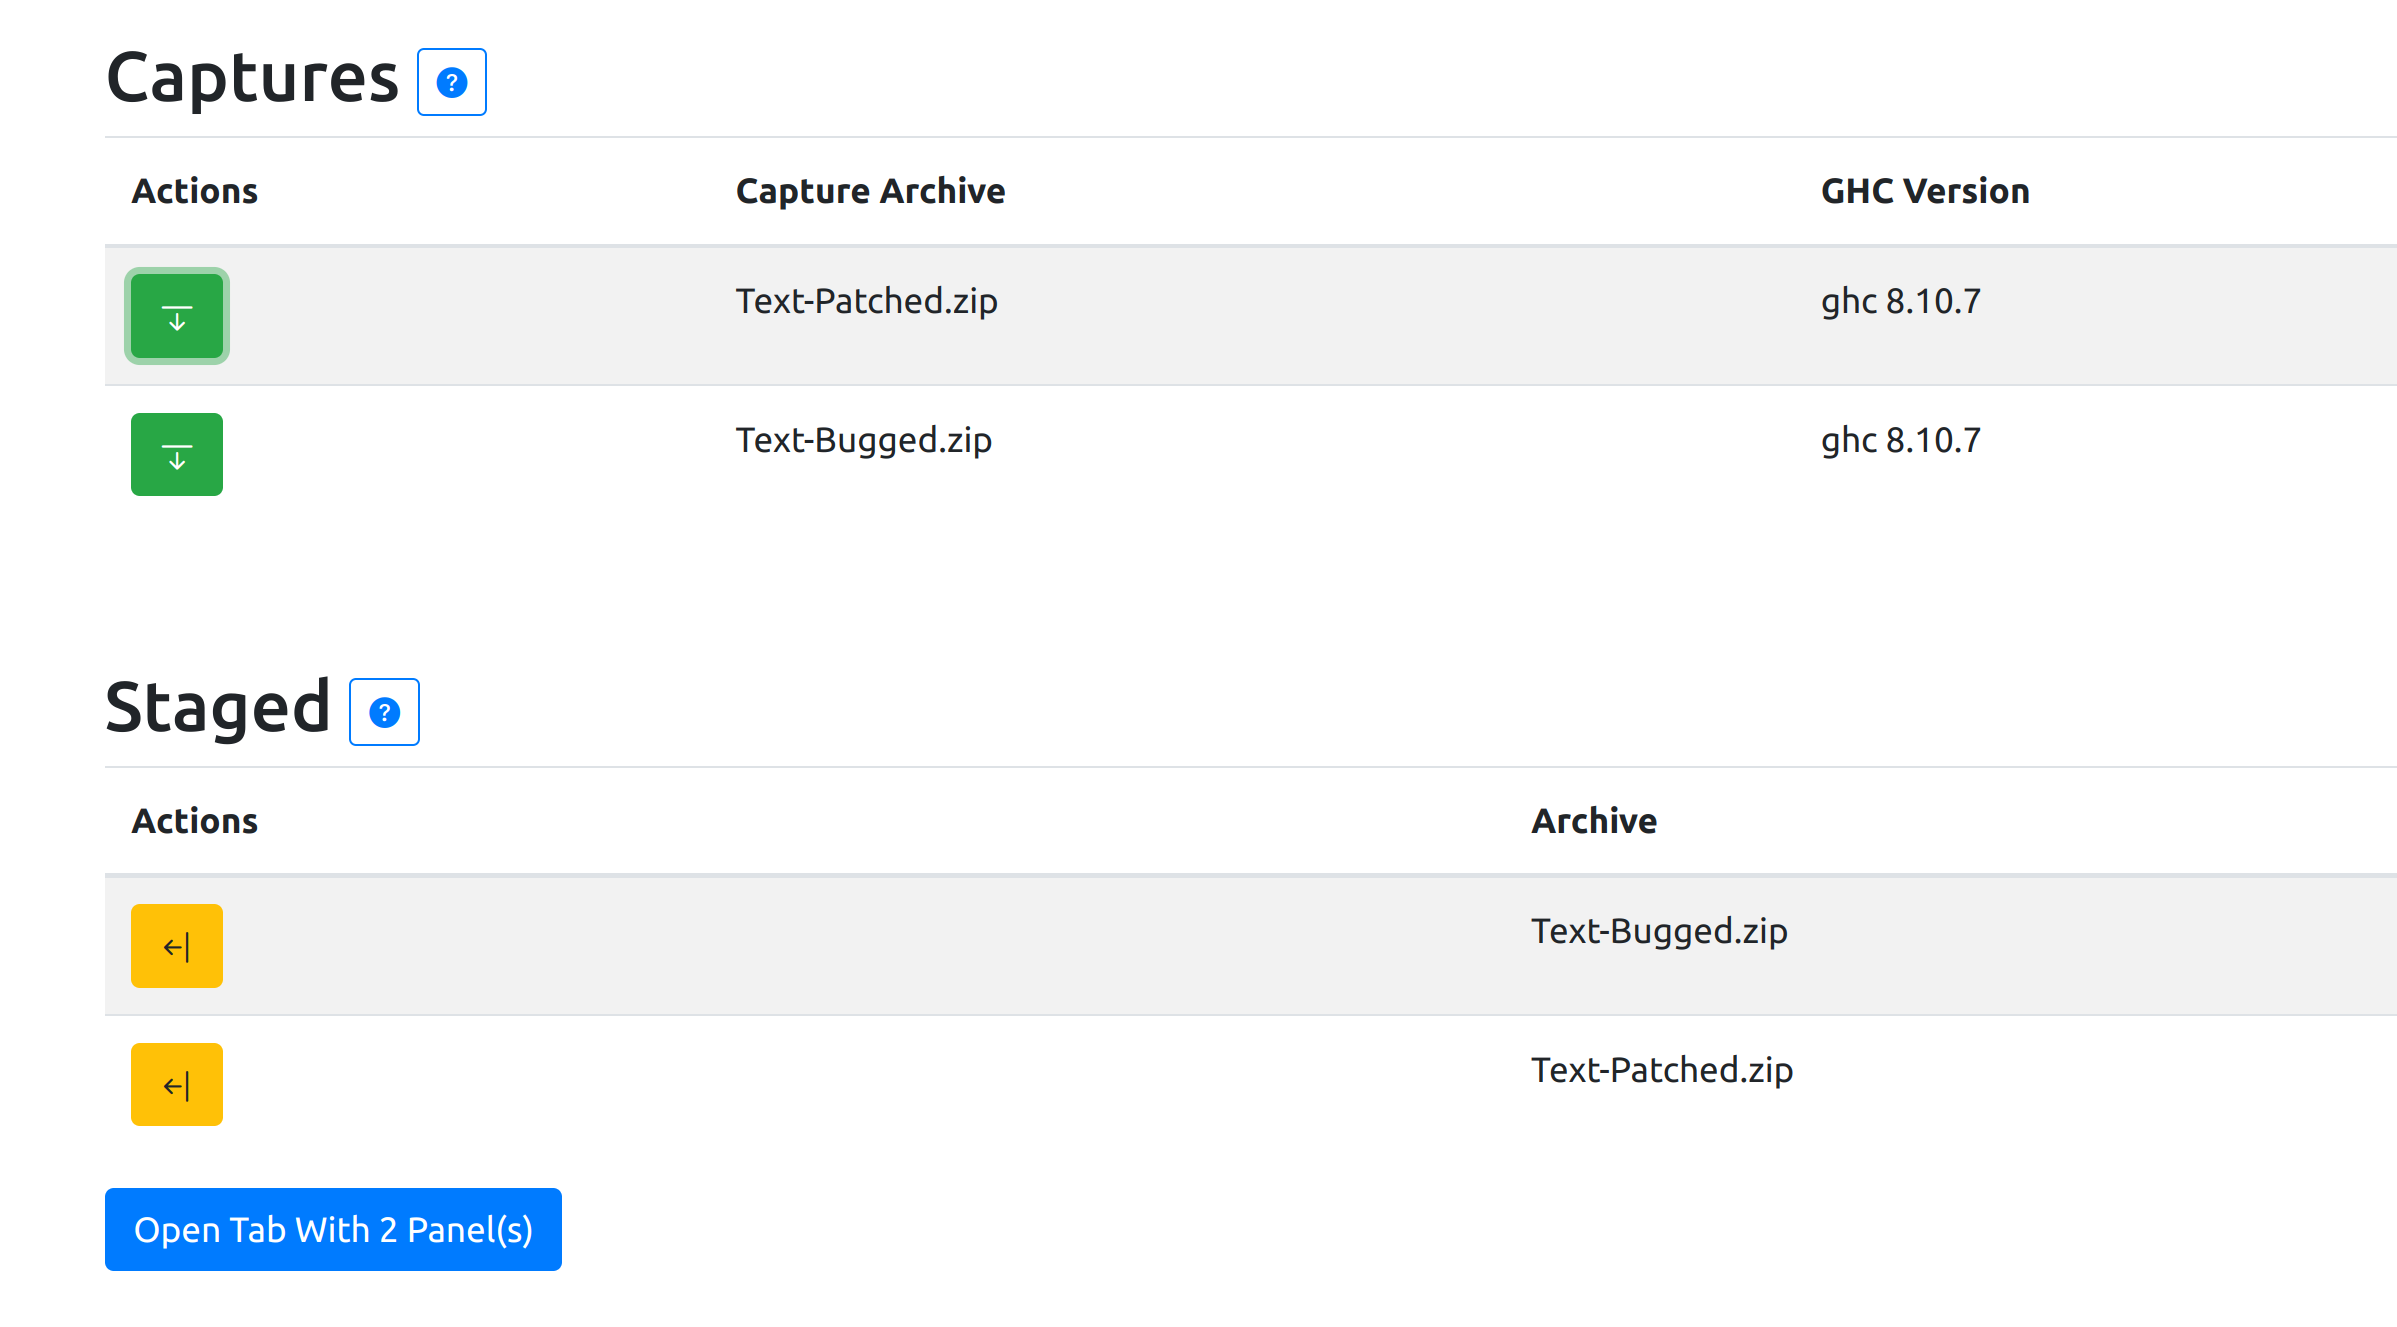
\includegraphics[width=0.8\textwidth]{figs/countchars_5.png}
\end{figure}

Because we now have more than 1 capture open at the same time we can use the \textit{Hide common definitions} feature to
find the first moment where the two captures converge. This happens to be at phase 1 of the simplifier pass:

\begin{figure}[H]
\centering
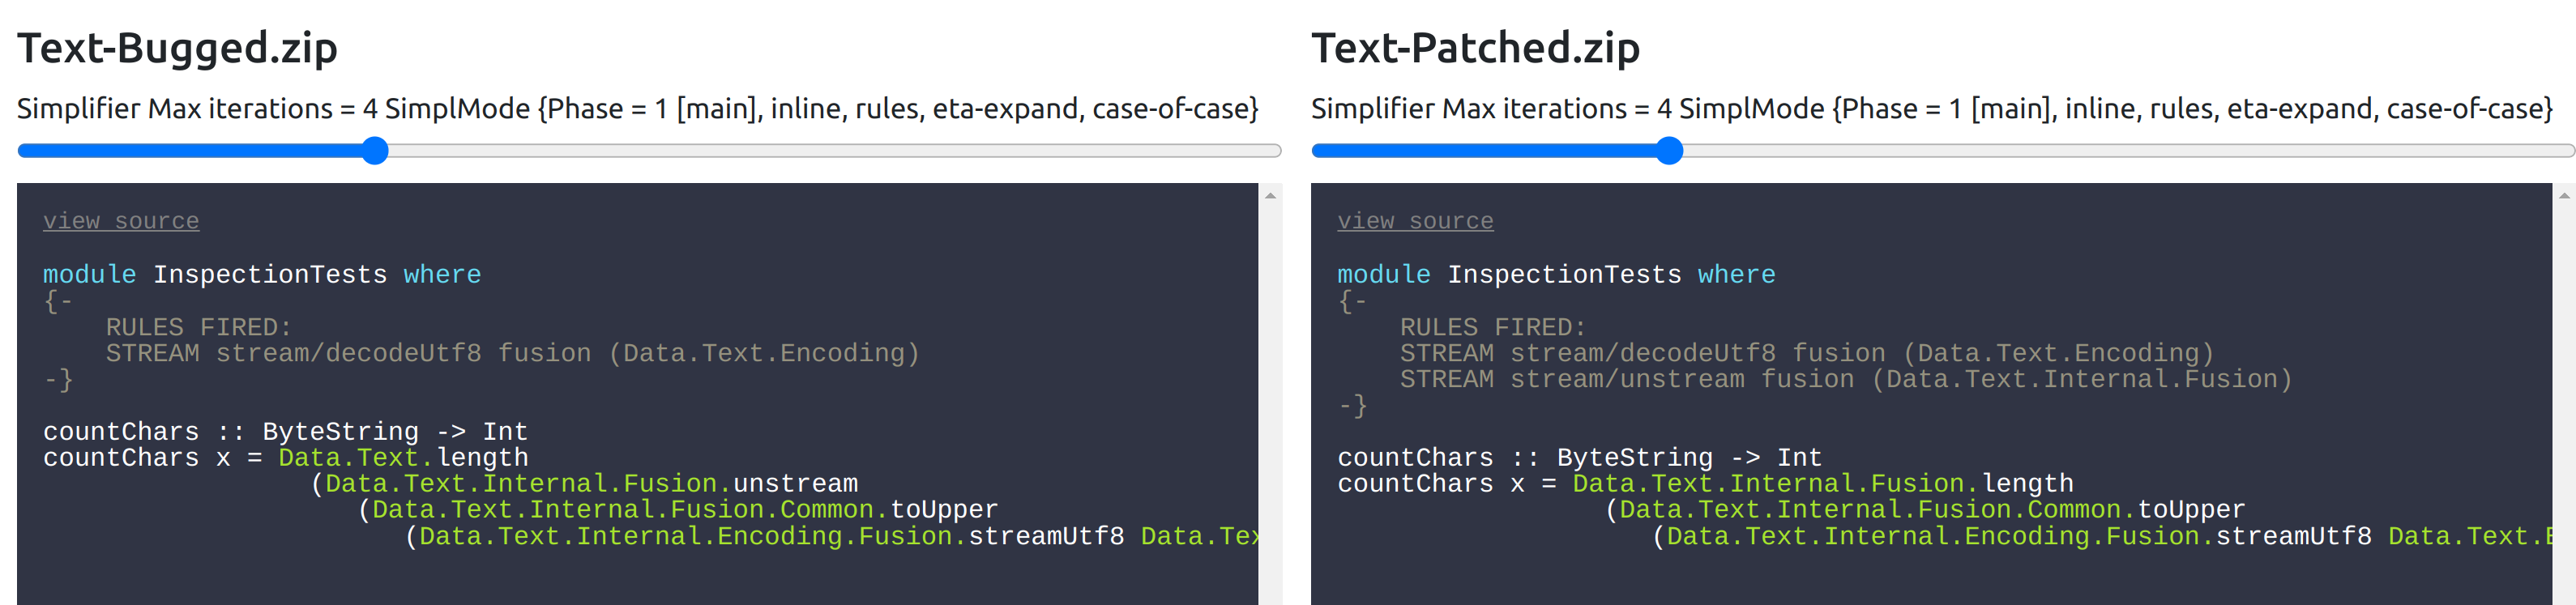
\includegraphics[width=0.9\textwidth]{figs/countchars_6.png}
\end{figure}

For clarity, let us extract the text from both panels and compare them:

\begin{listing}[H]
\begin{minted}[linenos,fontsize=\footnotesize]{haskell}
{-
    Text-Bugged.zip
    RULES FIRED:
    STREAM stream/decodeUtf8 fusion (Data.Text.Encoding)
-}

countChars :: ByteString -> Int
countChars x = Data.Text.length
                 (Data.Text.Internal.Fusion.unstream
                    (Data.Text.Internal.Fusion.Common.toUpper
                       (Data.Text.Internal.Encoding.Fusion.streamUtf8 Data.Text.Encoding.Error.strictDecode x)))

------------------------------------------------------------------
{-
    Text-Patched.zip
    RULES FIRED:
    STREAM stream/decodeUtf8 fusion (Data.Text.Encoding)
    STREAM stream/unstream fusion (Data.Text.Internal.Fusion)
-}

countChars :: ByteString -> Int
countChars x = Data.Text.Internal.Fusion.length
                 (Data.Text.Internal.Fusion.Common.toUpper
                    (Data.Text.Internal.Encoding.Fusion.streamUtf8 Data.Text.Encoding.Error.strictDecode x))
\end{minted}
\end{listing}

The most notable difference is the extra rewrite rule that was fired in the patched version (line 18).
Unfortunately, it is currently not possible to look up the definition of the rewrite rule in the tool itself, but
given that we know its name and originating module, we can find it in the source of \mono{text} without too much effort:

\begin{listing}[H]
\begin{minted}{haskell}
{-# RULES "STREAM stream/unstream fusion" forall s. stream (unstream s) = s #-}
\end{minted}
\end{listing}

From this we learn that at some point there was a stream/unstream pair to remove. Another difference is the module from which
the \mono{length} function is imported (\mono{Data.Text.Internal.Fusion.length} over \mono{Data.Text.length}). Like we predicted earlier,
the patched version uses a variant that operates directly on streams:

\begin{figure}[H]
\centering
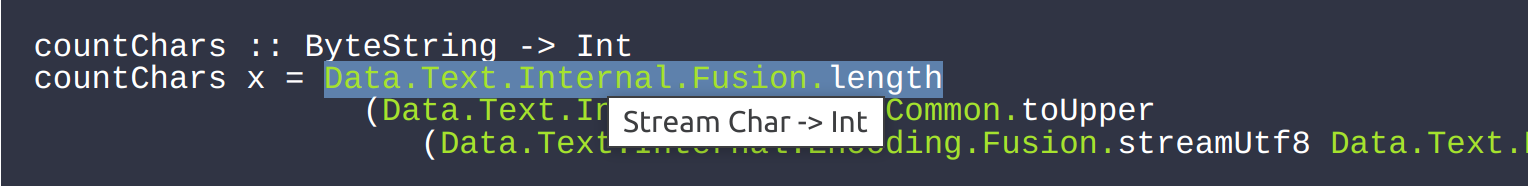
\includegraphics[width=0.8\textwidth]{figs/countchars_7.png}
\end{figure}

Given that in the previous in pass the captures were identical, and since no rewrite rule fired regarding \mono{length},
we can ascribe the difference to the inlining of \mono{length}. If we collect the definition of \mono{length} from both versions
of the text library we get:

\begin{listing}[H]
\begin{minted}{haskell}
-- Text-Bugged.zip
length :: Text -> Int
length t = S.length (stream t)
{-# INLINE [0] length #-}

-------------------------------------------

-- Text-Patched.zip
length :: Text -> Int
length t = S.length (stream t)
{-# INLINE [1] length #-}
\end{minted}
\end{listing}

The only difference is the phase annotation of the \mono{INLINE} pragma. The maintainers somehow decided that it was better
to inline \mono{length} one simplifier phase earlier (remember, phase 1 comes \textbf{before} phase 0). And they turned out to be right,
because inlining earlier uncovered the opportunity for the \textit{stream/unstream} rule to fire and remove 
the need to allocate an intermediate \mono{Text} value; Another exemplary manifestation of the Cascade Effect.

\paragraph{5. Epilogue: Brittleness of implicit fusion}
At or around the same time as Breitner. \cite{inspection_testing} identified the failed fusion case, Andrew Lelechenko had discovered
a problem involving the \mono{tail} function \cite{two_tails} under fusion. \mono{tail} just needs to drop the first character.
Despite needing to check whether to skip 1 or 2 bytes because of the UTF-16 encoding, this can be done in $O(1)$ time and memory.
Obviously this property should still hold when applying \mono{tail} twice in row. As it turns out, it does not. The following steps occur:

\begin{listing}[H]
\begin{minted}{haskell}
tail . tail
-- { inline to fusion variant }
unstream . S.tail . stream . unstream . S.tail . stream
-- { apply 'stream . unstream = id' }
unstream . S.tail . S.tail . stream
\end{minted}
\end{listing}

By constructing a stream we have become committed to traversing the entire structure where it was not needed at first,
yielding an $O(n)$ time and memory version after ``optimisation''. This is different from the situation in \mono{countChars},
where UTF-16 already dictated $O(n)$ runtime.

The ending to this story is quite simply that implicit fusion was disabled entirely \cite{two_tails} for similar functions.
Frequent \mono{text} contributor, Oleg Grenrus, remarked the following on the proposal to remove them:

\textit{``I think this is the right thing to do. Implicit fusion is unpredictable, and you explain, doesn't even work in simple cases.''}

Instead, users can now opt in by using the stream variant of such functions explicitly. This is a tragic example of how optimisation
can be unpredictable, and by extent, how people would favour predictability over automatic performance transformations that risk making the program slower.

\section{Lists vs Streams}

\begin{minted}{haskell}
Rec {
-- RHS size: {terms: 17, types: 17, coercions: 0, joins: 0/1}
Main.unlines [Occ=LoopBreaker]
  :: [GHC.Base.String] -> GHC.Base.String
[GblId, Arity=1, Str=<1L>, Unf=OtherCon []]
Main.unlines
  = \ (ds_s26z [Occ=Once1!] :: [[GHC.Types.Char]]) ->
      case ds_s26z of {
        [] -> GHC.Types.[] @GHC.Types.Char;
        : y_s26B [Occ=Once1] ys_s26C [Occ=Once1] ->
          let {
            sat_s26E [Occ=Once1, Dmd=ML] :: GHC.Base.String
            [LclId]
            sat_s26E = Main.unlines ys_s26C } in
          case GHC.Base.++ @GHC.Types.Char y_s26B Main.main5
          of sat_s26D [Occ=Once1]
          { __DEFAULT ->
          GHC.Base.++ @GHC.Types.Char sat_s26D sat_s26E
          }
      }
end Rec }

Rec {
-- RHS size: {terms: 17, types: 18, coercions: 0, joins: 0/1}
Main.unlines_go1 [Occ=LoopBreaker]
  :: [[GHC.Types.Char]] -> [GHC.Types.Char]
[GblId, Arity=1, Str=<1L>, Unf=OtherCon []]
Main.unlines_go1
  = \ (ds_s25d [Occ=Once1!] :: [[GHC.Types.Char]]) ->
      case ds_s25d of {
        [] -> GHC.Types.[] @GHC.Types.Char;
        : y_s25f [Occ=Once1] ys_s25g [Occ=Once1] ->
          let {
            sat_s25i [Occ=Once1, Dmd=ML] :: [GHC.Types.Char]
            [LclId]
            sat_s25i = Main.unlines_go1 ys_s25g } in
          case GHC.Base.++ @GHC.Types.Char y_s25f Main.main4
          of sat_s25h [Occ=Once1]
          { __DEFAULT ->
          GHC.Base.++ @GHC.Types.Char sat_s25h sat_s25i
          }
      }
end Rec }

\end{minted}




Here we discuss the basic of the stream paper, how it operates, why Haskell has not implemented it by favouring join points and
finally how the compilation pipeline treats these 2.

Perhaps repeat the unlines example from the background section.

\section{Erroneous program structure recovery in GHC fusion}
As part of our initial experiments to validate the tool, we decided to attempt to reproduce the shot-cut fusion of \mono{unlines} as presented
in the paper \cite{shortcut_fusion}. This serendipitously led to the discovery of a performance bug in GHC. Namely, the definition:

\begin{listing}[H]
\begin{minted}[linenos]{haskell}
unlines :: [String] -> String
unlines ls = concat (map (\l -> l ++ ['\n']) ls)
\end{minted}
\end{listing}

can be observed to be compiled to the following Core using our tool:

\begin{listing}[H]
\begin{minted}[linenos]{haskell}
cr_chr :: Char
cr_chr = C# '\n'

cr :: [Char]
cr = : cr_chr []

go1 :: [[Char]] -> [Char]
go1 ds = case ds of
  { : y ys -> ++
                (++ y cr)
                (go1 ys)
    [] -> []
  }

unlines :: [String] -> String
unlines ls = go1 ls
\end{minted}
\end{listing}

This definition is problematic because every line is first traversed to append a newline character and then again to append it to the rest of the line
yielding an $O(n^2)$ runtime, while we already know that an $O(n)$ runtime is possible. We can confirm that this version is indeed less performant by
benchmarking both \mono{unlines} and \mono{Prelude.unlines} on the first 73 lines of lorem ipsum:

\begin{listing}[H]
\begin{minted}{text}
benchmarking our_unlines
time                 127.9 μs   (125.0 μs .. 130.7 μs)
                     0.997 R²   (0.996 R² .. 0.998 R²)
mean                 126.6 μs   (124.6 μs .. 128.4 μs)
std dev              6.532 μs   (5.742 μs .. 7.504 μs)
variance introduced by outliers: 53% (severely inflated)

benchmarking prelude_unlines
time                 80.23 μs   (79.87 μs .. 80.53 μs)
                     1.000 R²   (0.999 R² .. 1.000 R²)
mean                 79.70 μs   (79.05 μs .. 80.13 μs)
std dev              1.858 μs   (1.088 μs .. 2.962 μs)
variance introduced by outliers: 20% (moderately inflated)
\end{minted}
\end{listing}

So it is clear that \mono{Prelude} has defined \mono{unlines} in a more efficient manner, but that does not take away the fact that any such
expression as our version of \mono{unlines} can reasonable expected to fuse in the most optimal manner. We investigate the reason for the suboptimal
fusion by using our tool. The tool reports that the following Core is desugared from the source:

\begin{listing}[H]
\begin{minted}[linenos]{haskell}
unlines :: [String] -> String
unlines ls = Data.Foldable.concat Data.Foldable.$fFoldable[]
               (GHC.Base.map
                  (\l -> GHC.Base.++ l
                           (GHC.Base.build
                              (\c n -> c
                                         (GHC.Types.C# '\n') n))) ls)
\end{minted}
\end{listing}

Here we can observe that the list literal \mono{['\n']} is already represented as a list producer function that is recognized nice with the short-cut fusion
rules. We can hypthesize in the near future \mono{map} and \mono{++} will be rewritten to their \textit{build/foldr} representation, making the fusion rule
applicable. After the first transformation, which is the also first pass of the simplifier, we get the following:

\begin{listing}[H]
\begin{minted}[linenos]{haskell}
unlines :: [String] -> String
unlines ls = GHC.Base.build
               (\c n -> GHC.Base.foldr
                          (GHC.Base.mapFB
                             (\x y -> GHC.Base.foldr c y x)
                             (\l -> GHC.Base.build
                                      (\c n -> GHC.Base.foldr c
                                                 (c
                                                    (GHC.Types.C# '\n') n) l))) n ls)
\end{minted}
\end{listing}

We can see how concat has been specialized and also rewritten, as well as \mono{++}. The result of \mono{map} however, is a bit more peculiar; contrary to what the paper
suggested at the time, we instead observe a call to some function \mono{mapFP}. The tool directly allows us to call upon Hoogle to find the definition of this function,
and the extensive documentation of the GHC Base library gives us some context:

\begin{listing}[H]
\begin{minted}[linenos]{haskell}
-- Note eta expanded
mapFB ::  (elt -> lst -> lst) -> (a -> elt) -> a -> lst -> lst
{-# INLINE [0] mapFB #-} -- See Note [Inline FB functions] in GHC.List
mapFB c f = \x ys -> c (f x) ys
\end{minted}
\end{listing}

\begin{listing}[H]
\begin{minted}[linenos]{text}
{- Note [The rules for map]
~~~~~~~~~~~~~~~~~~~~~~~~~~~
The rules for map work like this.

* Up to (but not including) phase 1, we use the "map" rule to
  rewrite all saturated applications of map with its build/fold
  form, hoping for fusion to happen.

  In phase 1 and 0, we switch off that rule, inline build, and
  switch on the "mapList" rule, which rewrites the foldr/mapFB
  thing back into plain map.

  It's important that these two rules aren't both active at once
  (along with build's unfolding) else we'd get an infinite loop
  in the rules.  Hence the activation control below.

* This same pattern is followed by many other functions:
  e.g. append, filter, iterate, repeat, etc. in GHC.List

  See also Note [Inline FB functions] in GHC.List

* The "mapFB" rule optimises compositions of map

* The "mapFB/id" rule gets rid of 'map id' calls.
  You might think that (mapFB c id) will turn into c simply
  when mapFB is inlined; but before that happens the "mapList"
  rule turns
     (foldr (mapFB (:) id) [] a
  back into
     map id
  Which is not very clever.

* Any similarity to the Functor laws for [] is expected.
-}

{-# RULES
"map"       [~1] forall f xs.   map f xs                = build (\c n -> foldr (mapFB c f) n xs)
"mapList"   [1]  forall f.      foldr (mapFB (:) f) []  = map f
"mapFB"     forall c f g.       mapFB (mapFB c f) g     = mapFB c (f.g)
"mapFB/id"  forall c.           mapFB c (\x -> x)       = c
  #-}
\end{minted}
\end{listing}

This documentation does not give us any insight yet into the role of the \mono{mapFB} function. Perhaps the note \mono{[Inline FB functions]} can provide
some more insight:

\begin{listing}[H]
\begin{minted}[linenos]{text}
Note [Inline FB functions]
~~~~~~~~~~~~~~~~~~~~~~~~~~

After fusion rules successfully fire, we are usually left with one or more calls
to list-producing functions abstracted over cons and nil. Here we call them
FB functions because their names usually end with 'FB'. It's a good idea to
inline FB functions because:

* They are higher-order functions and therefore benefits from inlining.

* When the final consumer is a left fold, inlining the FB functions is the only
  way to make arity expansion to happen. See Note [Left fold via right fold].

For this reason we mark all FB functions INLINE [0]. The [0] phase-specifier
ensures that calls to FB functions can be written back to the original form
when no fusion happens.

Without these inline pragmas, the loop in perf/should_run/T13001 won't be
allocation-free. Also see Trac #13001.
\end{minted}
\end{listing}

Here we find the answer to why \mono{mapFB} exists: ``\textit{alls to FB functions can be written back to the original form
when no fusion happens}''. It is desirable to retain the structure of the original map if it is not fused away. \mono{mapFB} enables does just that,
it exposes an initial opportunity to fuse but is reversible using the \textit{mapList} rule if no fusion happens. This has the convenient effect that 
compiled code can more closely represent the original source code on the hand, but on the other hand also limits code size.

Let's explore this further. If we always rewrite \mono{map} to  \mono{build (\c n -> foldr (\x r -> c (f x) r) n xs)}, then we lose some structure in the code.
Every loop will then generate a local, recursive loop. For example, take the function: \mono{addTwo = map (+1) . map (+1)}.

addTwo ds =
      case ds of
        [] -> []
        y : ys ->
          let xs = addTwo ys
              x = y+2
          in x:xs




addTwo1 x -> x+2

addTwo xs -> map addTwo1 xs



\begin{listing}[H]
\begin{minted}[linenos]{haskell}
\end{minted}
\end{listing}


% Trying to reach the same conclusion as https://github.com/haskell/text/issues/202 (recursing into the mentioned https://github.com/haskell/text/pull/348)

\section{Performance regression at Channable}

%https://github.com/haskell/text/issues/202
%https://github.com/haskell/text/pull/348
%
%Another performance regression: https://gitlab.haskell.org/ghc/ghc/-/issues/22207

\section{Comparison with existing tools}
